\documentclass[journal,12pt,twocolumn]{IEEEtran}
\usepackage{array,booktabs}
\newcommand\ml[1]{\multicolumn{1}{l}{#1}}
\newcommand\lparen{\mkern1mu(\mkern1mu}
\newcommand\rparen{\mkern1mu)\mkern1mu}
\newcommand\pp{\phantom{\lparen}}

\usepackage{setspace}
\usepackage{gensymb}
\singlespacing
\usepackage[cmex10]{amsmath}

\usepackage{amsthm}

\usepackage{mathrsfs}
\usepackage{txfonts}
\usepackage{stfloats}
\usepackage{bm}
\usepackage{cite}
\usepackage{cases}
\usepackage{subfig}

\usepackage{longtable}
\usepackage{multirow}

\usepackage{enumitem}
\usepackage{mathtools}
\usepackage{steinmetz}
\usepackage{tikz}
\usepackage{circuitikz}
\usepackage{verbatim}
\usepackage{tfrupee}
\usepackage[breaklinks=true]{hyperref}
\usepackage{graphicx}
\usepackage{tkz-euclide}
\usepackage{tabularx}

\usetikzlibrary{calc,math}
\usepackage{listings}
    \usepackage{color}                                            %%
    \usepackage{array}                                            %%
    \usepackage{longtable}                                        %%
    \usepackage{calc}                                             %%
    \usepackage{multirow}                                         %%
    \usepackage{hhline}                                           %%
    \usepackage{ifthen}                                           %%
    \usepackage{lscape}     
\usepackage{multicol}
\usepackage{chngcntr}
\usepackage{float}
\usepackage{polynom}
\makeatletter
\def\pld@CF@loop#1+{%
    \ifx\relax#1\else
        \begingroup
          \pld@AccuSetX11%
          \def\pld@frac{{}{}}\let\pld@symbols\@empty\let\pld@vars\@empty
          \pld@false
          #1%
          \let\pld@temp\@empty
          \pld@AccuIfOne{}{\pld@AccuGet\pld@temp
                            \edef\pld@temp{\noexpand\pld@R\pld@temp}}%
           \pld@if \pld@Extend\pld@temp{\expandafter\pld@F\pld@frac}\fi
           \expandafter\pld@CF@loop@\pld@symbols\relax\@empty
           \expandafter\pld@CF@loop@\pld@vars\relax\@empty
           \ifx\@empty\pld@temp
               \def\pld@temp{\pld@R11}%
           \fi
          \global\let\@gtempa\pld@temp
        \endgroup
        \ifx\@empty\@gtempa\else
            \pld@ExtendPoly\pld@tempoly\@gtempa
        \fi
        \expandafter\pld@CF@loop
    \fi}
\def\pld@CMAddToTempoly{%
    \pld@AccuGet\pld@temp\edef\pld@temp{\noexpand\pld@R\pld@temp}%
    \pld@CondenseMonomials\pld@false\pld@symbols
    \ifx\pld@symbols\@empty \else
        \pld@ExtendPoly\pld@temp\pld@symbols
    \fi
    \ifx\pld@temp\@empty \else
        \pld@if
            \expandafter\pld@IfSum\expandafter{\pld@temp}%
                {\expandafter\def\expandafter\pld@temp\expandafter
                    {\expandafter\pld@F\expandafter{\pld@temp}{}}}%
                {}%
        \fi
        \pld@ExtendPoly\pld@tempoly\pld@temp
        \pld@Extend\pld@tempoly{\pld@monom}%
    \fi}
\makeatother
\DeclareMathOperator*{\Res}{Res}

\renewcommand\thesection{\arabic{section}}
\renewcommand\thesubsection{\thesection.\arabic{subsection}}
\renewcommand\thesubsubsection{\thesubsection.\arabic{subsubsection}}

\renewcommand\thesectiondis{\arabic{section}}
\renewcommand\thesubsectiondis{\thesectiondis.\arabic{subsection}}
\renewcommand\thesubsubsectiondis{\thesubsectiondis.\arabic{subsubsection}}


\hyphenation{op-tical net-works semi-conduc-tor}
\def\inputGnumericTable{}                                 %%

\lstset{
%language=C,
frame=single, 
breaklines=true,
columns=fullflexible
}
\begin{document}


\newtheorem{theorem}{Theorem}[section]
\newtheorem{problem}{Problem}
\newtheorem{proposition}{Proposition}[section]
\newtheorem{lemma}{Lemma}[section]
\newtheorem{corollary}[theorem]{Corollary}
\newtheorem{example}{Example}[section]
\newtheorem{definition}[problem]{Definition}

\newcommand{\BEQA}{\begin{eqnarray}}
\newcommand{\EEQA}{\end{eqnarray}}
\newcommand{\define}{\stackrel{\triangle}{=}}
\bibliographystyle{IEEEtran}
\raggedbottom
\setlength{\parindent}{0pt}
\providecommand{\mbf}{\mathbf}
\providecommand{\pr}[1]{\ensuremath{\Pr\left(#1\right)}}
\providecommand{\qfunc}[1]{\ensuremath{Q\left(#1\right)}}
\providecommand{\sbrak}[1]{\ensuremath{{}\left[#1\right]}}
\providecommand{\lsbrak}[1]{\ensuremath{{}\left[#1\right.}}
\providecommand{\rsbrak}[1]{\ensuremath{{}\left.#1\right]}}
\providecommand{\brak}[1]{\ensuremath{\left(#1\right)}}
\providecommand{\lbrak}[1]{\ensuremath{\left(#1\right.}}
\providecommand{\rbrak}[1]{\ensuremath{\left.#1\right)}}
\providecommand{\cbrak}[1]{\ensuremath{\left\{#1\right\}}}
\providecommand{\lcbrak}[1]{\ensuremath{\left\{#1\right.}}
\providecommand{\rcbrak}[1]{\ensuremath{\left.#1\right\}}}
\theoremstyle{remark}
\newtheorem{rem}{Remark}
\newcommand{\sgn}{\mathop{\mathrm{sgn}}}
\providecommand{\abs}[1]{\left\vert#1\right\vert}
\providecommand{\res}[1]{\Res\displaylimits_{#1}} 
\providecommand{\norm}[1]{\left\lVert#1\right\rVert}
%\providecommand{\norm}[1]{\lVert#1\rVert}
\providecommand{\mtx}[1]{\mathbf{#1}}
\providecommand{\mean}[1]{E\left[ #1 \right]}
\providecommand{\fourier}{\overset{\mathcal{F}}{ \rightleftharpoons}}
%\providecommand{\hilbert}{\overset{\mathcal{H}}{ \rightleftharpoons}}
\providecommand{\system}{\overset{\mathcal{H}}{ \longleftrightarrow}}
	%\newcommand{\solution}[2]{\textbf{Solution:}{#1}}
\newcommand{\solution}{\noindent \textbf{Solution: }}
\newcommand{\cosec}{\,\text{cosec}\,}
\providecommand{\dec}[2]{\ensuremath{\overset{#1}{\underset{#2}{\gtrless}}}}
\newcommand{\myvec}[1]{\ensuremath{\begin{pmatrix}#1\end{pmatrix}}}
\newcommand{\mydet}[1]{\ensuremath{\begin{vmatrix}#1\end{vmatrix}}}
\numberwithin{equation}{subsection}
\makeatletter
\@addtoreset{figure}{problem}
\makeatother
\let\StandardTheFigure\thefigure
\let\vec\mathbf
\renewcommand{\thefigure}{\theproblem}
\def\putbox#1#2#3{\makebox[0in][l]{\makebox[#1][l]{}\raisebox{\baselineskip}[0in][0in]{\raisebox{#2}[0in][0in]{#3}}}}
     \def\rightbox#1{\makebox[0in][r]{#1}}
     \def\centbox#1{\makebox[0in]{#1}}
     \def\topbox#1{\raisebox{-\baselineskip}[0in][0in]{#1}}
     \def\midbox#1{\raisebox{-0.5\baselineskip}[0in][0in]{#1}}
\vspace{3cm}
\title{CBSE Maths 10, 2019}
\maketitle
\newpage
\tableofcontents
\bigskip
\renewcommand{\thefigure}{\theenumi}
\renewcommand{\thetable}{\theenumi}

%Get Python codes from 
%%
%\begin{lstlisting}
%https://github.com/gadepall/cbse-papers/2007/math/10/solutions/codes
%\end{lstlisting}
%%
%Get latex-tikz codes from 
%%
%\begin{lstlisting}
%https://github.com/gadepall/cbse-papers/2007/math/10/solutions
%\end{lstlisting}
\section{Discrete maths}
\renewcommand{\theequation}{\theenumi}
\begin{enumerate}[label=\thesection.\arabic*.,ref=\thesection.\theenumi]
\numberwithin{equation}{enumi}
\item If in an A.P., $a$ = 15, $d$= -3, and $a_n$ = 0. Find $n$ value. \\
\solution We know that $a_n$ = $a+(n-1)d$,
\begin{align}
& 0 = 15+ (n-1)(-3) \nonumber \\
& 3(n-1) = 15 \nonumber \\ 
& n = 6 \nonumber 
\end{align}

\item If $S_n$, the sum of first $n$ terms of an A.P.,is given by $S_n = 2n^2+n$ then find its $n^{th}$ term\\
\solution We know that $S_n - S_{n-1} = n^{th}$ term\\
Given $S_n = 2n^2+n$, 
\begin{align}
& S_n = 2n^2+n \nonumber \\
& S_{n-1} = 2(n-1)^2+(n-1) \nonumber \\
& S_n - S_{n-1} = (2n^2+n) - (2(n-1)^2+(n-1)) \nonumber \\
& n^{th} term = 4n-1 \nonumber
\end{align}
\item If the $17^{\text{th}}$ of an A.P., exceeds $10^{\text{th}}$ term by 7, then fine the common difference.  \\
\solution We know that $a_n$ = $a+(n-1)d$\\Given $a_{17} - a_{10} = 7$
\begin{align}
& a_{17} = a+16d \nonumber \\
& a_{10} = a+9d \nonumber \\
& a_{17} - a{10} = 7d = 7 \nonumber \\
& d =1 \nonumber
\end{align}
\item If in an A.P., the $n^{th}$ term is $\dfrac{1}{m}$ and $m^{th}$ is given by $\dfrac{1}{n}$. Find \\
(i) $(mn)^{th}$ term\\
(ii) Sum of the first $(mn)$ terms \\
\solution We know that $a_n$ = $a+(n-1)d$, $a_m = \dfrac{1}{n}$, $a_n = \dfrac{1}{m}$
\begin{align}
& a+(m-1)d = \dfrac{1}{n}  \label{1}\\
& a+(n-1)d = \dfrac{1}{m} \\ 
& \myvec{1 & m-1 \\ 1 & n-1} \myvec{a\\d} = \myvec{\dfrac{1}{n} \\ \dfrac{1}{m}} \nonumber \\
& \myvec{a+(m-1)d \\ a+(n-1)d} = \myvec{\dfrac{1}{n} \\ \dfrac{1}{m}} \nonumber 
\end{align}
Considering the augmented matrix
\begin{align}
 & \myvec{a+(m-1)d&\dfrac{1}{n} \\ a+(n-1)d&\dfrac{1}{m}}& \nonumber \\
 &\xleftrightarrow[]{ R_2 \leftarrow R_1 - R_2}
 &\myvec{a+(m-1)d&\dfrac{1}{n} \\ (m-n)d&\dfrac{m-n}{mn}}& \\
 &d = \dfrac{1}{mn} \nonumber
 \medskip \nonumber 
\end{align}
 Substituting in \eqref{1} we get \\ 
 $a = \dfrac{1}{mn}$\\
\begin{enumerate}
\item
 \begin{align}
 & a_{mn} = a+(mn-1)d \nonumber \\
 & a_{mn} = (\dfrac{1}{mn})+(mn-1)(\dfrac{1}{mn}) \nonumber \\
 & a_{mn} = 1 \nonumber
 \end{align}
\item
 \begin{align}
 & S_{n} =  n(\dfrac{a+l}{2})\nonumber \\
 & S_{mn} =  mn(\dfrac{a+l}{2})\nonumber \\
 & S_{mn} =  \dfrac{1+mn}{2}\nonumber\\
 \nonumber
 \end{align}
\end{enumerate}

\item Find the HCF of 612 and 1314 \\
\solution 
\[
\setlength\arraycolsep{0pt}
\begin{array}{ *{11}{r} }
   612 & \rparen & 1314 & \lparen & \ml{2} \\
   &&        1224 & \pp \\
\cmidrule{3-4}
   && 90 & \rparen & 612 & \lparen & \ml{6} \\
   &&&& 540 & \pp \\
\cmidrule{5-6}
   &&&& 72 & \rparen & 90 & \lparen & \ml{1} \\
   &&&&&& 18 & \pp \\
\cmidrule{7-8}
   &&&&&& 18 & \rparen & 72 & \lparen & \ml{4} \\
   &&&&&&&& 72 & \pp\\
\cmidrule{9-10}
   &&&&&&&& \multicolumn{2}{c}{\times}
\end{array}
\] \\
The HCF of 612 \& 1314 is 18 
\item Show that $5 - 3\sqrt{2}$ is an irrational number, where $\sqrt{2}$ is given to be an irrational number.\\
\item Show that any positive integer is of the form $6m+1$ or $6m+3$ or $6m+5$, where m is some integer.
\end{enumerate}
\section{Probability and Statistics}
\renewcommand{\theequation}{\theenumi}
\begin{enumerate}[label=\thesection.\arabic*.,ref=\thesection.\theenumi]
\numberwithin{equation}{enumi}
\item A die has 6 faces having the letters A,B,C,A,A,B. The die is thrown once. What is the probability of getting (i) A (ii) B.\\ 
\solution \\
Total no. of faces on the die =6 \\
No. of faces having A on it = 3 \\
No. of faces having B on it = 2\\ 
Therefore, \\
P(A)=  $\dfrac{\text{No. of faces having A}}{\text{Total no. of faces}} = \dfrac{3}{6} = \dfrac{1}{2}$ \\ \\ \\
P(B)=  $\dfrac{\text{No. of faces having B}}{\text{Total no. of faces}} = \dfrac{2}{6} = \dfrac{1}{3}$ \\ \\
\item Find the probability that a number selected at random from the numbers 3,4,4,4,5,5,6,6,6,7 will be their mean.\\
\solution \\
Mean = $\dfrac{3+4+4+4+5+5+6+6+6+7}{10}$ = 5\\
P(5) = $\dfrac{2}{10}$ = $\dfrac{1}{5}$\\ \\
\item Find the mode of the following frequency distribution:\\
\begin{table}[ht]
 \centering
 \resizebox{\columnwidth}{!}{
 \begin{tabular}{ |c|c|c|c|c|c|c|c| } 
 \hline
  Class: & 10-14 & 14-18 & 18-22 & 22-26 & 26-30 & 30-34 & 34-38 \\
 \hline
 Frequency: & 8 & 6 & 11 & 20 & 25 & 22 & 10  \\
 \hline
\end{tabular}}
 \caption{}
 \end{table} \\
\solution 
Here, maximum frequency is 25.\\
Modal class is 26-30.\\
So, $l=26,f_0 = 20, f_1 = 25, f_2 = 22, h = 4$ \\
Mode = $l+(\dfrac{f_1 - f_0}{2f_1-f_0-f_2}) h$ \\
Mode = 28.5\\
\item For the following frequency distribution, obtain frequency distribution curve and hence obtain the median.\\
\begin{table}[ht]
 \centering
 \resizebox{\columnwidth}{!}{
 \begin{tabular}{ |c|c|c|c|c|c|c|c| } 
 \hline
  Class: & 0-10 & 10-20 & 20-30 & 30-40 & 40-50 & 50-60 & 60-70 \\
 \hline
 Frequency: & 5 & 15 & 20 & 23 & 17 & 11 & 9  \\
 \hline
\end{tabular}}
 \caption{}
 \end{table} \\
\solution \\
\begin{figure}[h]
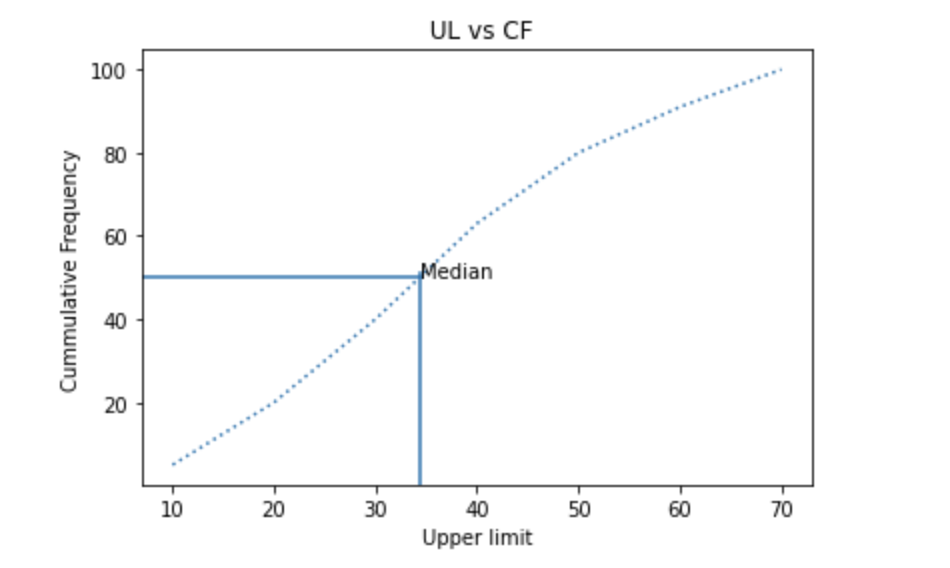
\includegraphics[width= 100mm]{hi}
\end{figure}\\
Median occurs as 34.3 \\
\item Find the values of frequencies x and y in the following frequency distribution table if N=100, and median = 32.\\
\begin{table}[ht]
 \centering
 \resizebox{\columnwidth}{!}{
 \begin{tabular}{ |c|c|c|c|c|c|c|c| } 
 \hline
  Marks: & 0-10 & 10-20 & 20-30 & 30-40 & 40-50 & 50-60 & Total \\
 \hline
 No. of students: & 10 & x & 25 & 30 & y & 10 & 100  \\
 \hline
\end{tabular}}
 \caption{}
 \end{table} \\
\solution 
\begin{table}[ht]
 \centering
 \resizebox{\columnwidth}{!}{
 \begin{tabular}{ |c|c|c|c|c|c|c|c| } 
 \hline
  Marks: & 0-10 & 10-20 & 20-30 & 30-40 & 40-50 & 50-60 & Total \\
 \hline
 No. of students: & 10 & x & 25 & \textbf{30} & y & 10 & 100  \\
 \hline
 Cumm Freq: & 10 & 10+x & 35+x & 65+x & 65+x+y & 75+x+y & 75+x+y = 100 \\
 \hline
\end{tabular}}
 \caption{}
 \end{table} \\


$75+x+y=100\\
x+y=25 \\
f=30,h=10,c_f=35+x,\dfrac{N}{2} =50$\\
Median = $ l+ \dfrac{(N/2)- c_f}{f} h$\\
$32 = 30 + (\dfrac{50-35-x}{30})10$\\
$x=9$\\
$y=16$ 
\end{enumerate}
\section{Linear Algebra}
\renewcommand{\theequation}{\theenumi}
\begin{enumerate}[label=\thesection.\arabic*.,ref=\thesection.\theenumi]
\numberwithin{equation}{enumi}
\item The area of two similar triangles are 25 sq.cm and 121 sq.cm. Find the ratio of their corresponding sides. \\
\solution \\
We know that,the ratio of area of two similar triangles is equal to the squares of the ratio of two corresponding sides.\\
Let, 'a' cm and 'b' cm be the lengths of the corresponding sides of the two triangles with area 25 sq. cm and 121 sq. cm respectively.\\
Then, we must have\\
$\dfrac{25}{121} = \dfrac{a^2}{b^2}$\\ \\
$\dfrac{5}{11} = \dfrac{a}{b}$\\ \\
The ratio of their corresponding sides is 5:11.\\
 \begin{figure}
	  \centering 
	  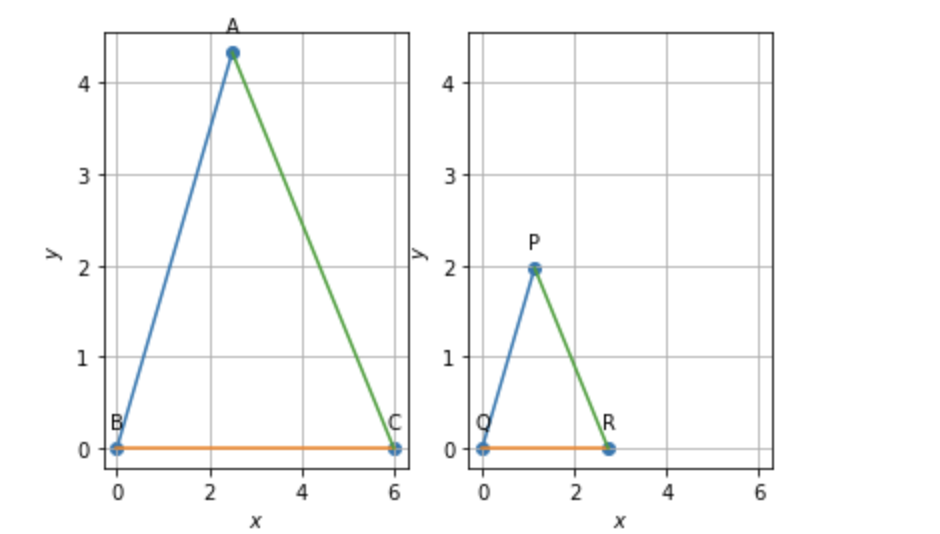
\includegraphics[width=\columnwidth]{3.1}
	  \caption{}
	  \label{fig:geometry-3.9.pdf}
 \end{figure}\\ 
\item Find the values of for which the distance between the point A $\myvec{x\\2}$ and B $\myvec{9\\8}$ is 10.\\
\solution \\
In 2D space the distance derived from $L^2$ norm. \\
$||A-B||$ = $\sqrt{\myvec{A-B}^T\myvec{A-B}}$\\
$(A-B) = \myvec{x-9 \\ -6} $\\
$||A-B||$ = $\sqrt{\myvec{x-9 \\ -6}\myvec{x-9 & -6}}$\\
$||A-B||$ = $\sqrt{(x-9)^2+36}$\\
$10 = \sqrt{x^2-18x+117}$\\
$x^2-18x+17 = 0$\\
$(x-17)(x-1) = 0$\\
Thus, the values of x are 17,1.\\
 \begin{figure}
	  \centering 
	  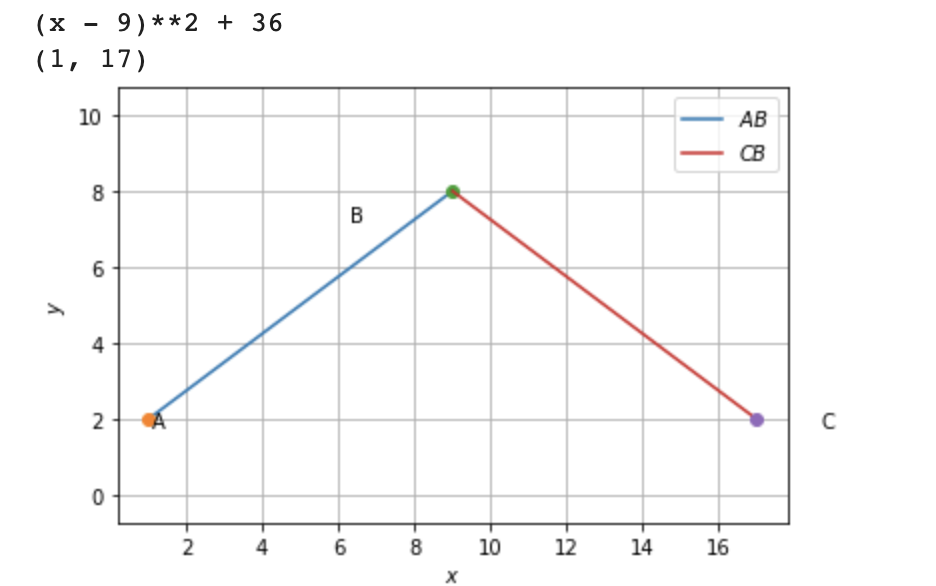
\includegraphics[width=\columnwidth]{3.2}
	  \caption{}
	  \label{fig:geometry-3.9.pdf}
 \end{figure}\\ 
\item A juice seller was serving his customers using glass. The inner diameter of the cylindrical glass was 5 cm , but the bottom of the glass had a hemispherical raised portion which reduced the capacity of the glass. If the height of the glass was 10 cm, find what the apparent capacity of the glass was and what the actual capacity was ?.\\
\solution Given,that the bottom of the glass had a hemispherical raised portion which reduced the capacity of the glass.\\
\begin{table}[ht]
 \centering
 \resizebox{\columnwidth}{!}{
 \begin{tabular}{ |c|c|c| } 
 \hline
 Symbol & Description & Value\\
 \hline
 D & inner diameter & 5 cm \\
 \hline
 h & height of glass & 10 cm \\
 \hline
 r & radius & $\frac{D}{2}$ = 2.5 cm \\
 \hline
 $V_{app}$ & apparent volume & ? \\
 \hline
 $V_{actual}$ & actual volume & ? \\
 \hline
\end{tabular}}
 \caption{}
 \end{table} \\
Actual capacity of Glass= Volume of cylinder - Volume of hemisphere.\\
$V_{app} = \pi r^2 h$\\
$V_{app} = \pi (2.5^2) (10)$\\
$V_{app} = 196.25cm^3$\\
Volume of hemisphere = $\frac{2}{3} \pi r^3$\\
Volume of hemisphere = $\frac{2}{3} \pi (2.5)^3$\\
Volume of hemisphere = $32.7cm^3$\\
$V_{actual}$ = $196.25cm^3 -32.7cm^3 $\\
$V_{actual}$ = $163.55cm^3$\\
\item A girl empties a cylindrical bucket, full of sand, of base radius 18 cm and height 32 cm on the floor to form a conical heap of sand. if the height of this conical heap  is 24 cm, then find its slant height correct up to one place of decimal. \\
\solution Given, \\
\begin{table}[ht]
 \centering
 \resizebox{\columnwidth}{!}{
 \begin{tabular}{ |c|c|c| } 
 \hline
 Symbol & Description & Value\\
 \hline
 $r_1$ & base radius & 18 cm \\
 \hline
 $h_1$ & height of bucket & 32 cm \\
 \hline
 $h_2$ & height of cone &  24 cm \\
 \hline
 l & slant height of cone & $\sqrt {h_2^2 +r_2^2}$=? \\
 \hline
\end{tabular}}
 \caption{}
 \end{table} \\
Volume of sand in Cylindrical bullet = Volume of conical head of sand\\
$\pi r_1^2 h_1 = \frac{1}{3} \pi r_2^2 h_2$\\ \\
$r_2^2 = \dfrac{18*18*32*3}{24}$\\
$r_2 = 36$\\
Slant height =  $\sqrt {h_2^2 +r_2^2}$ \\
Slant height =  $\sqrt {24^2 +36^2}$\\
Slant height =  43.2cm



\item An open metal bucket is in the shape of frustum of a cone, mounted on a hollow cylindrical base made of the same metallic sheet. The diameter of the two circular end of buckets are 45 cm and 25 cm, the total vertical height of the bucket is 24 cm, find the area of metallic sheet used to make the bucket. Also find the volume of the water it can hold.
\solution Given, \\
\begin{table}[ht]
 \centering
 \resizebox{\columnwidth}{!}{
 \begin{tabular}{ |c|c|c| } 
 \hline
 Symbol & Description & Value\\
 \hline
 $r_1$ & First radius & 22.5 cm \\
 \hline
 $r_2$ & Second radius & 12.5 cm \\
 \hline
 $h$ & height of frustum cone & 24 cm \\
 \hline
\end{tabular}}
 \caption{}
 \end{table} \\ 
 l = Slant height of the frustum cone. \\
 
 Slant height =  $\sqrt {h^2 +(r_1-r_2)^2}$ \\
 Slant height =  $\sqrt {24^2 +(22.5-12.5)^2}$ \\
 Slant height = 26cm\\
 
Area of metallic sheet used=Curved surface area of the frustum of cone+area of circular base+curved surface area of cylinder. \\

Area of metallic sheet used = $\pi(r_1-r_2)l+\pi r_2^2$\\
Area of metallic sheet used = $1307.7 cm^2$\\

Volume of water that the bucket can hold = $\frac{1}{3} \pi(r_1^2 + r_2^2 + r_1r_2)h$\\

Volume of water that the bucket can hold  = $23719.02cm^3$ \\

\item The mid-point of the line segment joining A $\myvec{2a\\4}$ and B $\myvec{-2\\3b}$ is P $\myvec{1\\2a+1}$. The values of a and b are .\\ 
\solution:
Given, P as mid point which is $\dfrac{A+B}{2}$\\
$A+B = \myvec{2a\\4} + \myvec{-2\\3b}$ \\ \\
$\dfrac{A+B}{2} =  \myvec{a-1\\1.5b+2} = P$ \\
$ \myvec{a-1\\1.5b+2} = \myvec{1\\2a+1} $ \\
$ a -1 =1$ ; \\
$a =2 $ \\
$1.5b+2 = 2a+1 ; 1.5b+2 = 5;\\
b = 2 $ \\
   \begin{figure}
	  \centering 
	  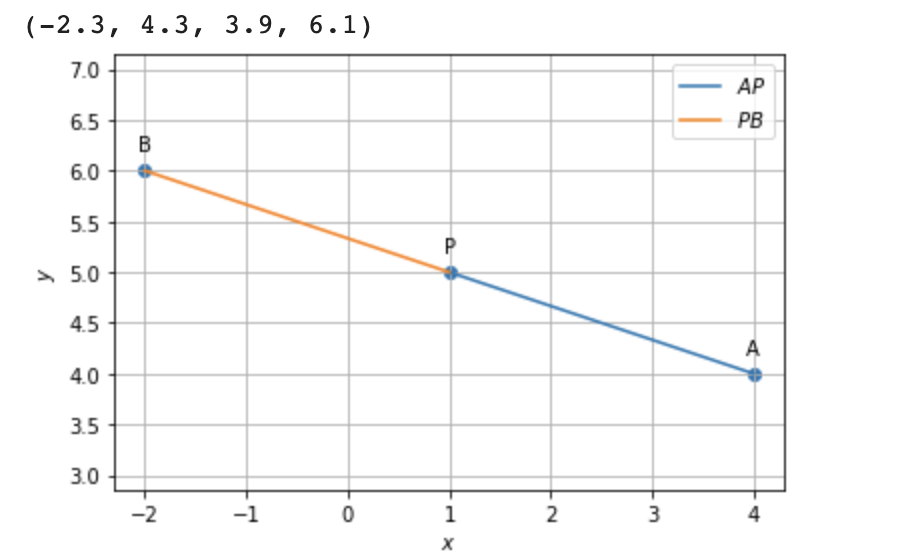
\includegraphics[width=\columnwidth]{3.6}
	  \caption{Line segment P as mid point}
	  \label{fig:geometry-3.9.pdf}
  \end{figure}

\item For what value of p, are the points A $\myvec{2\\1}$, B $\myvec{p\\-1}$, P $\myvec{-1\\3}$ are collinear. \\
\solution The equation of a line passing through a point is given by \begin{align}\vec{n}^T\vec{x}=c \label{1} \end{align}
From \eqref{1} The equation of the line passing through points $\vec{A}, \vec{B}, \vec{C}$ is given by:
\begin{align}
\vec{n}^T\vec{A}=c \label{2} \\
\vec{n}^T\vec{B}=c \label{3 }\\
\vec{n}^T\vec{C}=c \label{4} 
\end{align}
if the points are collinear then 
\begin{align}
\vec{B-A}^T\vec{n} = 0 \\
\vec{C-B}^T\vec{n} = 0 \\
\myvec{\vec{B-A} & \vec{C-B}}^T\vec{n} = 0 \label{5}
\end{align}
Considering $\eqref{5}$
\begin{align}
\myvec{p-2 & -(1+p) \\ -2 & 4}^T\vec{n} = 0 \nonumber \\
\myvec{p-2 & -2 \\ -(1+p) & 4}^T\vec{n} = 0 \label{6}
\end{align}
Since, $\vec{n}$ is non zero, \eqref{6} must be 
\[
\begin{vmatrix}
p-2 & -2 \\ 
-(1+p) & 4
\end{vmatrix}
= 0
\] \\
$[(p-2)*4] - [2*(1+p)] = 0 $ \\
Solving this we get \textbf{p=5}

   \begin{figure}
	  \centering 
	  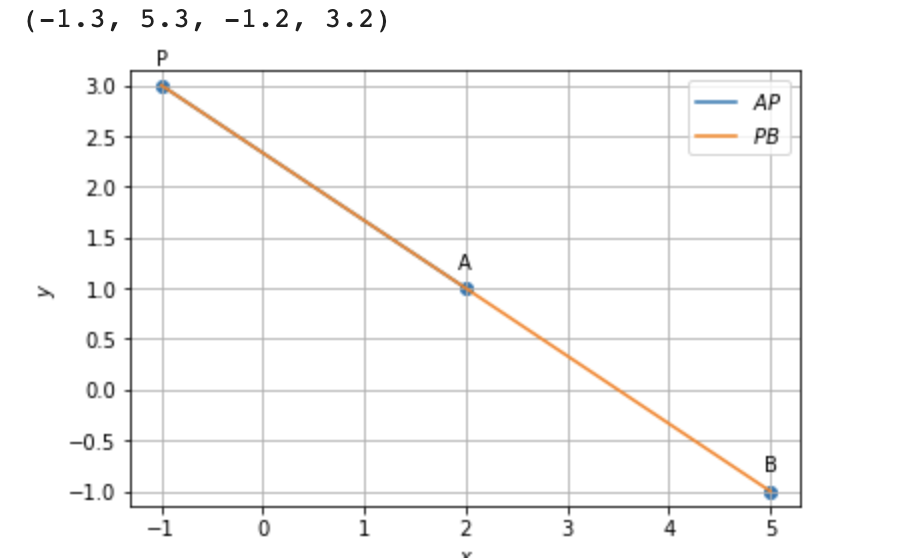
\includegraphics[width=\columnwidth]{3.7}
	  \caption{Collinear points}
	  \label{fig:geometry-3.9.pdf}
  \end{figure}

\item Point P divides the line segment joining the points A $\myvec{2 \\1}$ B $\myvec{5 \\ -8}$ such that $\dfrac{AP}{AB}$ = $\dfrac{1}{3}$. If P lies on the line $2x-y+k = 0$ , find the value of k.\\
\solution Given $\dfrac{AP}{AB} =\dfrac{1}{3} $  \\
$\dfrac{AP}{AP+PB} =\dfrac{1}{3} $ \\


From this we get, \\
$\dfrac{AP}{PB} =\dfrac{1}{2} $\\

Consider the line  \begin{align}\myvec{-2& 1}\vec{x}=k \label{7}\end{align} which is in the form 
\begin{align}\vec{n}^T\vec{x}=c \label{8} \end{align}
 divides the line segment $\vec{A}$ and $\vec{B} $ in $1:2$ ratio, which means $s = 2$. 
$\vec{P} $ is point of intersection of two lines.\\ 
From the section formula we can write,
\begin{align}
&\vec{P} = \dfrac{1}{s+1}\left[\vec{B}+ s\vec{A}\right]& \nonumber \\
 \end{align} 
$ \vec{P} = \myvec{3 \\ -2}$ \\
The point $\vec{P}$ passes through the line $\vec{n}^T\vec{x}=c$, therefore,
\begin{align}
&\vec{n}^T\vec{P}=c& \nonumber\\
&\vec{n}^T\left(\displaystyle\frac{\vec{B}+s\vec{A}}{s+1} \right)=k& \label{0}
\end{align}
Solving for k from \eqref{7} and \eqref{8}, we get,
\begin{align}
& \vec{n}^T = \myvec{-2&1}& \nonumber\\
& \vec{A} = \myvec{2 \\1}& \nonumber\\
& \vec{B} = \myvec{5\\-8} \nonumber
\end{align}
Substituting the above values in \eqref{0} we get,
\begin{align}
& k =\myvec{2 & -1}\dfrac{\myvec{5 \\ -8} + 2 \myvec{2 \\1}}{3} & \nonumber \\
&k = 8 \nonumber
\end{align}
Therefore, the value of k is 8.\\
   \begin{figure}
	  \centering 
	  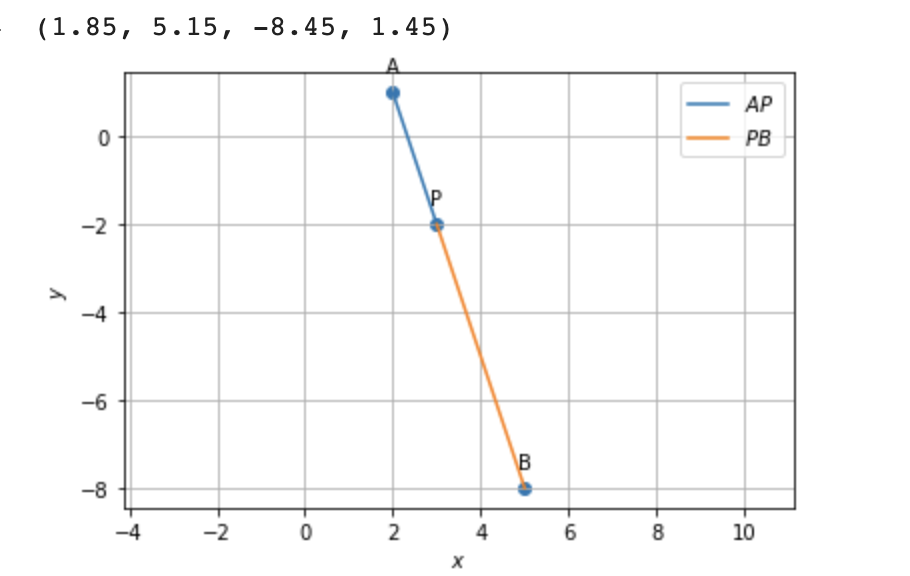
\includegraphics[width=\columnwidth]{3.9}
	  \caption{}
	  \label{fig:geometry-3.9.pdf}
  \end{figure}

\item In the figure $\angle AOB$ = 60 \textdegree, $\angle EOF$ = 80 \textdegree, $\angle COD$ = 40\textdegree and radius of the circle is 7cm. Find the area of the sectors for which angles are given.


\begin{table}[ht]
 \centering
 \resizebox{\columnwidth}{!}{
 \begin{tabular}{ |c|c| } 
 \hline
  Input Parameters & Output Parameters \\
 \hline
  r=7cm &  $\theta_3$ = 90\textdegree\\
 \hline
  O = $\myvec{0 \\ 0}$ &  $\vec{A}$ = $\myvec{r \\ 0}$, $\vec{B}$ = $\myvec{r \cos 60  \\ -r\sin60 }$  \\
 \hline
 $\theta_1$ = 30\textdegree & $\vec{C}$ = $\myvec{r \cos (60+ \theta_1)  \\ -r\sin(60+\theta_1) }$, $\vec{D}$ = $ \myvec{r \cos (60+40+\theta_1)  \\ -r\sin (60+40+\theta_1) }$  \\
 \hline 
 $\theta_2$ = 60\textdegree & $\vec{E}$ = $\myvec{r \cos (80+\theta_3)  \\ r\sin (80+\theta_3) }$, $\vec{F}$ = $  \myvec{0 \\ r}$ \\
 \hline
\end{tabular}}
 \caption{}
 \end{table} 
\solution: Given angles are $\angle AOB$ = 60 \textdegree, $\angle EOF$ = 80 \textdegree, $\angle COD$ = 40\textdegree, sum of the angles = 180 \textdegree. \\
Area of sector = $\dfrac{\theta \text{\textdegree}}{360 \text{\textdegree}} * \pi r^2$ \\
Area of the sectors for which angles are given is $ \dfrac{\pi}{2}* r^2$ \\
 \begin{figure}
	  \centering 
	  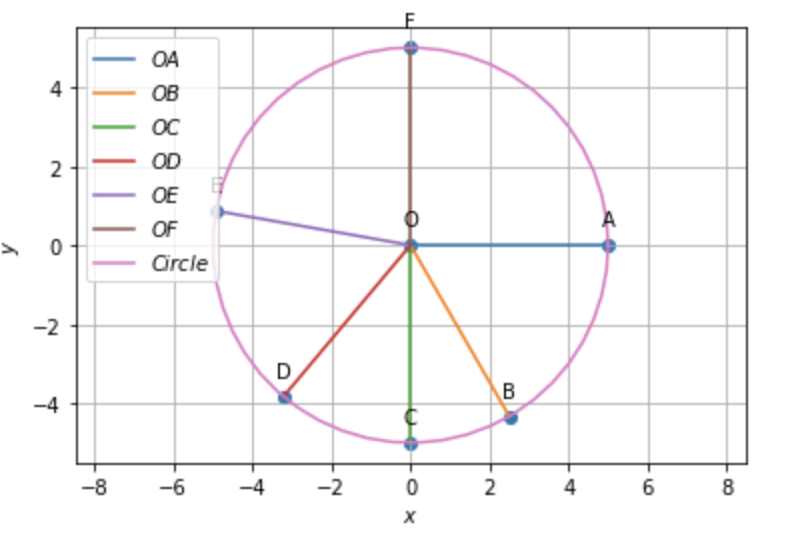
\includegraphics[width=\columnwidth]{sectors}
	  \caption{Circles and Sectors}
	  \label{fig:geometry-3.9.pdf}
 \end{figure}\\ 
\item Construct a pair of tangents to a circle of radius 4 cm which are inclined to each other at 60\textdegree. \\
\solution: 
\begin{table}[ht]
 \centering
 \resizebox{\columnwidth}{!}{
 \begin{tabular}{ |c|c|c| } 
 \hline
  Symbol & Value & Description \\
 \hline
 r & 4 & radius of the circle\\
 \hline
 d & 8 & Distance of $\vec{P}$ from the origin \\
 \hline
 $\sin \theta$ & $\dfrac{r}{d}$ & Angle between tangent from $\vec{P}$ and d\\ 
 \hline
 $\vec{P}$ & $\vec{0}$ & Origin \\
 \hline
 $\vec{O}$ & $\myvec{d \\ 0}$ & Centre of the circle\\
 \hline
 $\vec{Q_i}$ & $r \cot\theta\myvec{\cos\theta \\ \pm\sin\theta}$ & Points of contact \\
 \hline
\end{tabular}} 
 \caption{}
 \end{table} 
 \begin{figure}
	  \centering 
	  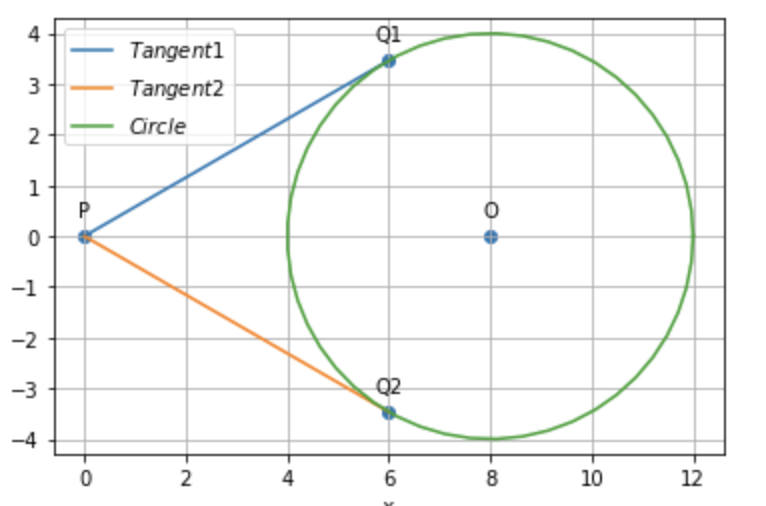
\includegraphics[width=\columnwidth]{tans}
	  \caption{Pair of Tangents to a Circle}
	  \label{fig:geometry-3.9.pdf}
 \end{figure}\\ 
 

\item In $\vec{\Delta}$ABC, $\angle$ B = 90\textdegree\;and D is the mid-point of BC. Prove that
$AC^2 = AD^2 + 3CD^2$.\\
\begin{table}[ht]
 \centering
 \resizebox{\columnwidth}{!}{
 \begin{tabular}{ |c|c| } 
 \hline
  Input Parameters & Output Parameters \\
 \hline
  a=3 &  $\vec{C}$ = $\myvec{a \\ 0}$\\
 \hline
  c=4 &  $\vec{A}$ = $\myvec{0 \\ c}$ \\
 \hline
  $\vec{B}$ = $\myvec{0 \\ 0}$ & $\vec{D}$ = $\vec{\dfrac{C}{2}}$\\
 \hline 
\end{tabular}}
 \caption{}
 \end{table}
  \begin{figure}
	  \centering 
	  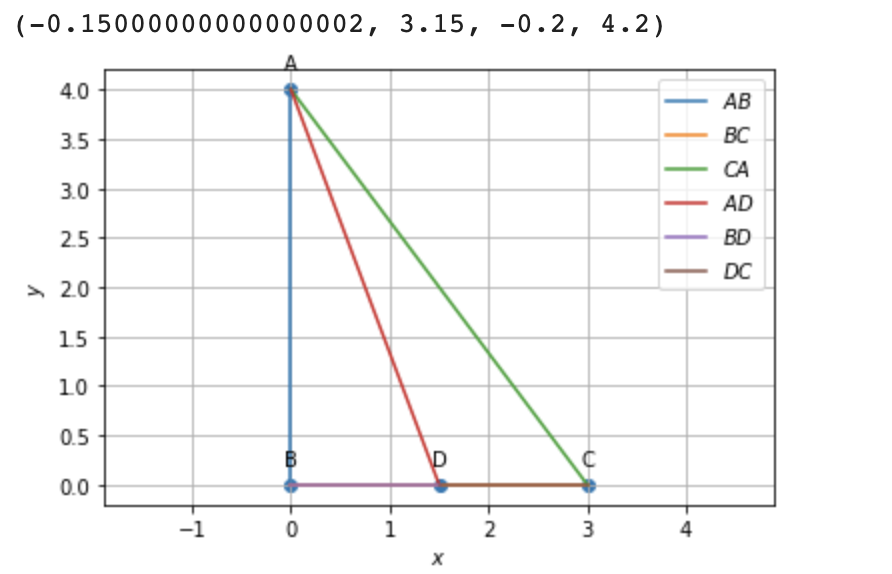
\includegraphics[width=\columnwidth]{tri1}
	  \caption{Triangle 1}
	  \label{fig:geometry-3.9.pdf}
  \end{figure}
\item In Figure, E is a point on CB produced of an isosceles $\vec{\Delta}$ ABC, with side
AB = AC. If AD $\perp$ BC and EF $\perp$ AC, prove that $\triangle ABD \sim \triangle ECF$.
\begin{table}[ht]
 \centering
 \resizebox{\columnwidth}{!}{
 \begin{tabular}{ |c|c| } 
 \hline
  Input Parameters & Output Parameters \\
 \hline
  a=4 &  $ \vec{C}$ = $\myvec{a \\ 0}$\\
 \hline
  $\vec{B}$ = $\myvec{0 \\ 0}$ & $\vec{D}$ = $\vec{\dfrac{C}{2}}$, $\theta_1 = \cos ^{-1} (\dfrac{a}{2c})$\\
 \hline 
  c=5 &  $\vec{A}$ = $\myvec{c\cos \theta_1 \\ c\sin \theta_1}$ \\
 \hline
 s = 3 & $\vec{E}$ = $\myvec{-s \\ 0}$, $\vec{F}$ = $\myvec{0.84a, \sin (\dfrac{b}{3})}$\\
 \hline
\end{tabular}}
 \caption{}
 \end{table}
   \begin{figure}
	  \centering 
	  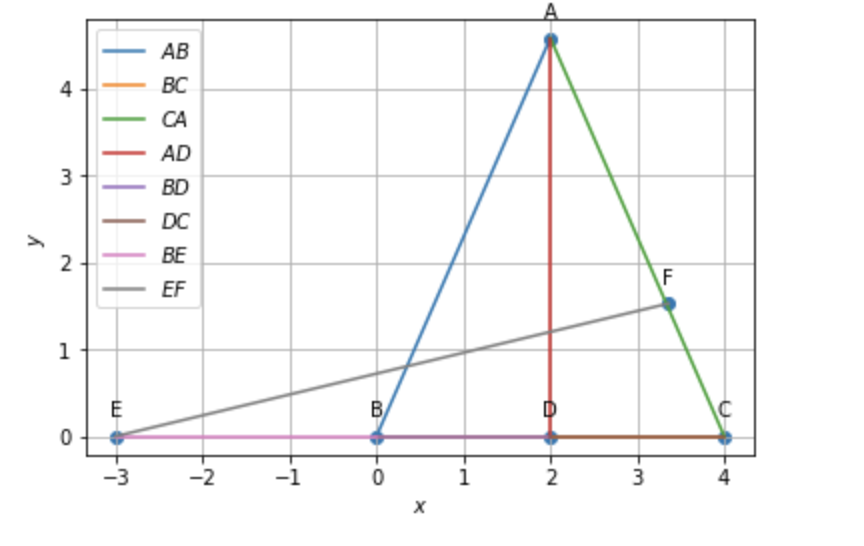
\includegraphics[width=\columnwidth]{Tri2}
	  \caption{Triangle 2}
	  \label{fig:geometry-3.9.pdf}
  \end{figure} 
\item In two concentric circles, prove that all chords of the outer circle which touch the inner circle, are of equal length.\\
\solution Norm of  $||x|| = c$, where $\vec{x}$ is the contact point on the circle. \\
Considering $||px||^2 = (px)^T (px)$\\
$p = \myvec{\cos \theta & -\sin \theta \\ \sin \theta & \cos \theta}$ \\
$p^T = \myvec{\cos \theta & \sin \theta \\ -\sin \theta & \cos \theta}$\\
$||px||^2 = ||x||^2 . I$\\
Which states that norm is unchanged with respect to the rotation, hence we can say that all chords of the outer circle which touch the inner circle, are of equal length.
   \begin{figure}
	  \centering 
	  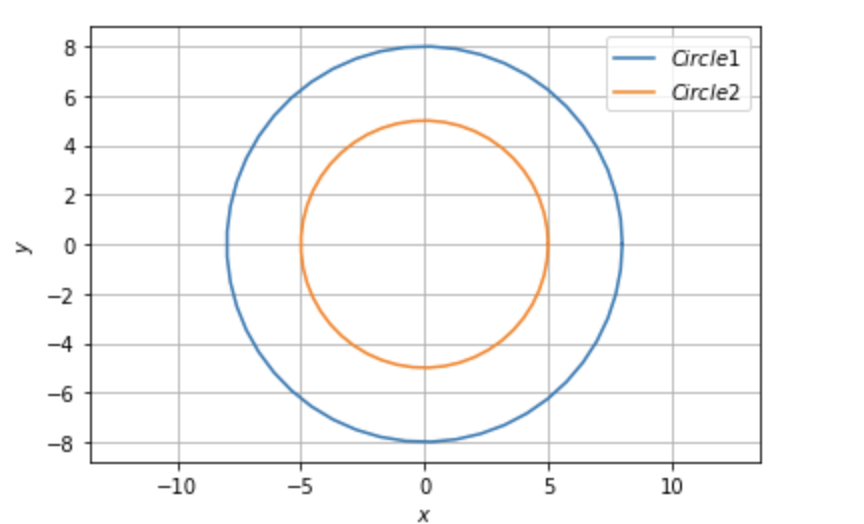
\includegraphics[width=\columnwidth]{3.13}
	  \caption{Circles with radius 8 \& 5}
	  \label{fig:geometry-3.9.pdf}
  \end{figure} 

 

  

\end{enumerate}

\section{Trigonometry}
\renewcommand{\theequation}{\theenumi}
\begin{enumerate}[label=\thesection.\arabic*.,ref=\thesection.\theenumi]
\numberwithin{equation}{enumi}
\item A boy standing on a horizontal plane finds a bird, flying at a distance of 100 m from him at an elevation of 30\textdegree . A girl standing on the roof of a 20 m high building finds the angle of elevation of the same bird to be 45\textdegree. Both the boy and the girl are on the opposite side of the bird. Find the distance of the bird from the girl.\\
\begin{table}[ht]
 \centering
 \resizebox{\columnwidth}{!}{
 \begin{tabular}{ |c|c| } 
 \hline
  Input Parameters & Output Parameters \\
 \hline
  a = 4 &  $\vec{B}$ = $\myvec{a \\ 0}$ \\
 \hline
 s = 2 &  $\vec{F}$ = $\myvec{a+s \\ 0}$, $\vec{A}$ = $\myvec{a  \\ a\tan \theta }$  \\
 \hline
 $\theta$ = 30\textdegree & $\vec{D}$ = $\myvec{a  \\ 0.4 a\tan \theta }$ \\
 \hline 
 $\vec{C}$ = $\myvec{0 \\ 0}$ & $\vec{E}$ = $\myvec{a+s \\ 0.4 a\tan \theta }$ \\
 \hline
\end{tabular}}
 \caption{}
 \end{table} 

 \begin{figure}
	  \centering 
	  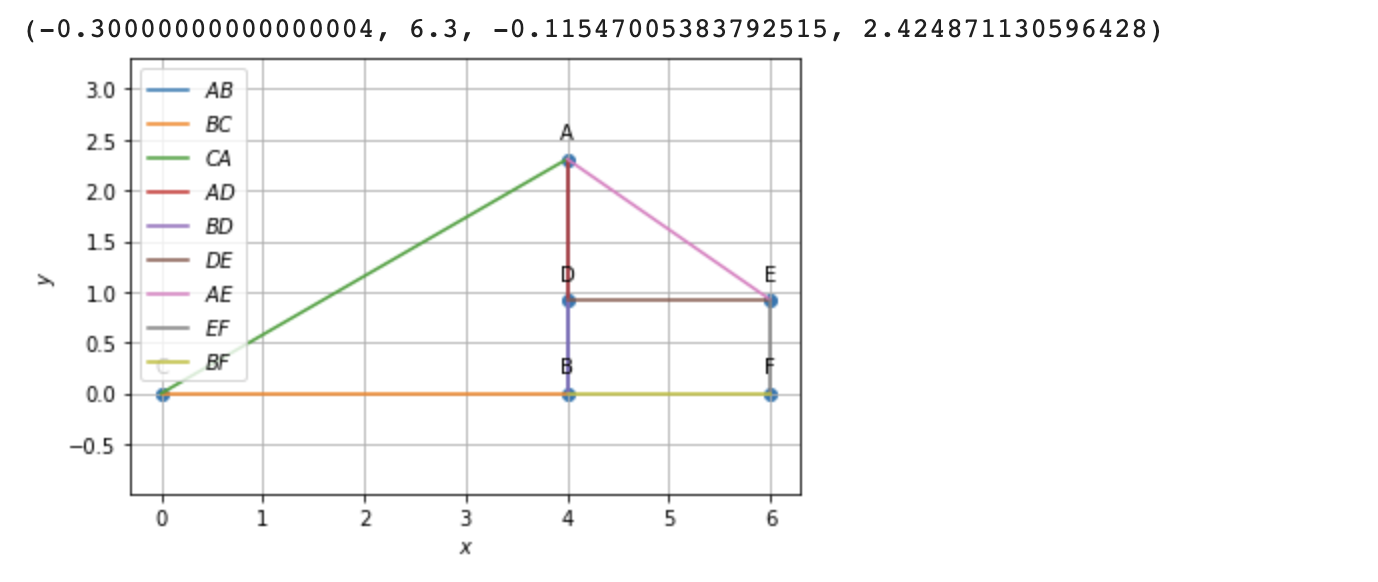
\includegraphics[width=\columnwidth]{4.1}
	  \caption{}
	  \label{fig:geometry-3.9.pdf}
 \end{figure}

\solution Let A be the position of the bird and E and C be the positions of the girl and the boy, respectively. \\

$\angle ACB$=30\textdegree ,$\angle AED$=45\textdegree AC=100 m,EF=20 m \\

In the $\triangle ACB$ we have\\

$ \sin 30\textdegree = \dfrac{AB}{AC}$ \\  

AB = 50m\\
AD = AB -BD\\
AD = 50-EF = 50-20 = 30m \\
In the $\triangle ADE$ we have\\

$ \sin 45\textdegree = \dfrac{AD}{AE}$ \\ 

AE = 43.2m \\
Therefore, the distance of bird from the girl is 42.3 m.\\
\begin{figure}
	\centering 
	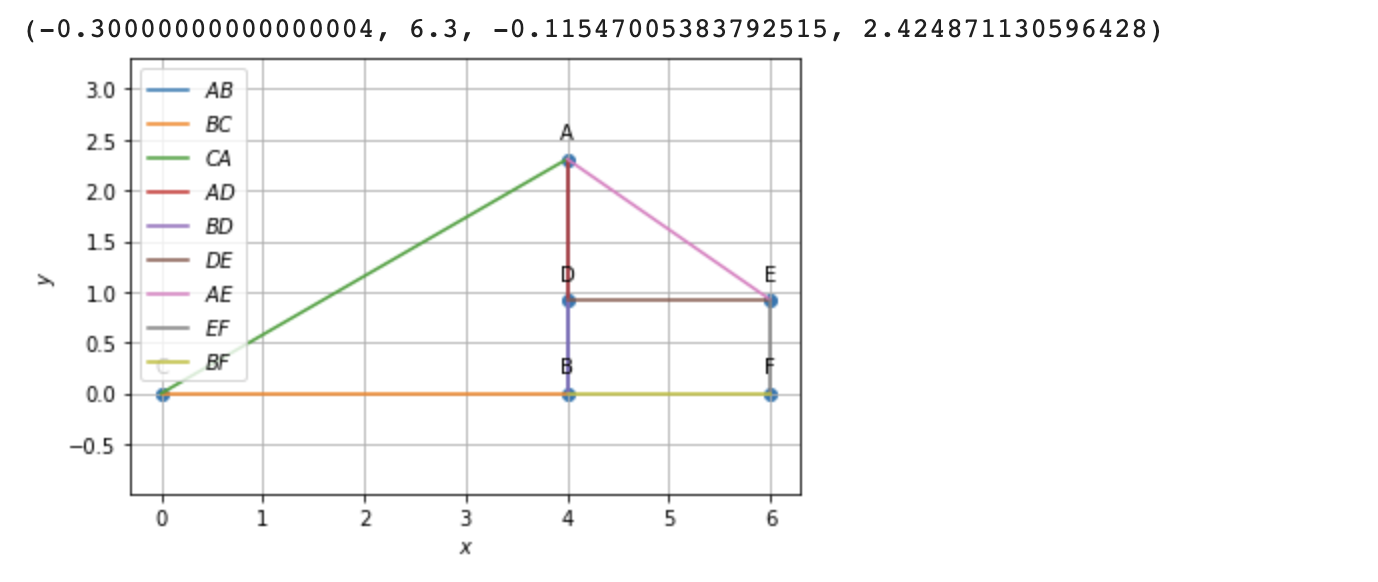
\includegraphics[width=\columnwidth]{4.1}
	\caption{}
\end{figure} 

\item The angle of elevation of an aeroplane from a point on the ground is 60\textdegree. After a flight of 30 seconds, the angle of elevation changes to 30\textdegree. If the aeroplane is flying at a height of 3600$\sqrt{3}$ m, then find the speed of the plane.\\
\begin{table}[ht]
 \centering
 \resizebox{\columnwidth}{!}{
 \begin{tabular}{ |c|c| } 
 \hline
  Input Parameters & Output Parameters \\
 \hline
  a = 4 &  $\vec{B}$ = $\myvec{a/\tan \theta_1 \\ 0}$ \\
 \hline
 $\theta_1$ = 45\textdegree &  $\vec{C}$ = $\myvec{a/\tan \theta_1 \\ a}$  \\
 \hline
 $\theta_2$ = 30\textdegree & $\vec{E}$ = $\myvec{a/\tan \theta_2 \\ a}$ \\
 \hline 
 $\vec{A}$ = $\myvec{0 \\ 0}$ & $\vec{D}$ = $\myvec{a/\tan \theta_2 \\ 0}$ \\
 \hline
\end{tabular}}
 \caption{}
 \end{table} 

 \begin{figure}
	  \centering 
	  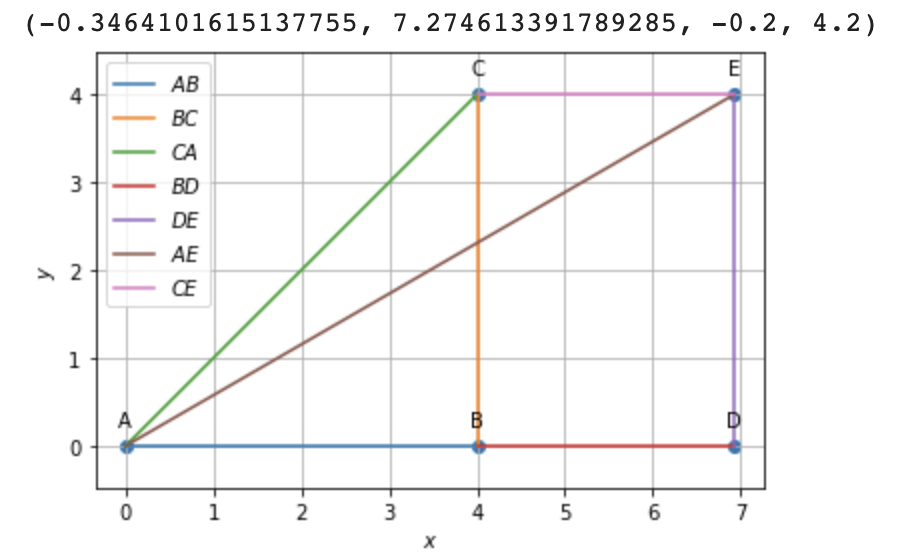
\includegraphics[width=\columnwidth]{4.2}
	  \caption{}
	  \label{fig:geometry-3.9.pdf}
 \end{figure}

\solution Let A be the point on the ground and the distance CE be the distance travelled by plane in 30 seconds. So,\\

In the $\triangle ACB$ we have\\

$ \tan 60$\textdegree = $\dfrac{BC}{AB}$ \\  

$\sqrt{3} = \dfrac{3600\sqrt{3}}{AB}$ \\

AB = 3600m \\

In the $\triangle ADE$ we have\\

$ \tan 30$\textdegree = $\dfrac{DE}{AD}$ \\  

$\dfrac{1}{\sqrt{3}} = \dfrac{3600\sqrt{3}}{AD}$ \\

AD = 10800m \\
Distance travelled = AD - AB = 10800-3600 = 7200 \\
Speed is: \\

$\dfrac{\text{Distance travelled}}{\text{Time taken}} = \dfrac{7200}{30}$ = 240m/s. \\



\item Prove that 
\begin{align}
& \dfrac{\tan \theta}{1- \tan \theta} - \dfrac{\cot \theta}{ 1- \cot \theta} = \dfrac{\cos \theta + \sin \theta}{\cos \theta - \sin \theta} \nonumber&
\end{align}\\
\solution Replace $\cot \theta$ \text{with} $\dfrac{1}{\tan \theta}$ \\
\begin{align}
& \dfrac{\tan \theta}{1- \tan \theta} - \dfrac{\dfrac{1}{\tan \theta}}{ 1- \dfrac{1}{\tan \theta}}  \nonumber& \\
& \dfrac{1+ \tan \theta}{1- \tan \theta}& \nonumber 
\end{align}
Converting them into $\sin \theta$ and $\cos \theta$ terms we get 
$ \dfrac{\cos \theta + \sin \theta}{\cos \theta - \sin \theta}$\\
Hence proved. \\
\item If $\cos \theta + \sin \theta = \sqrt{2} \cos \theta$, show that $\cos \theta - \sin \theta = \sqrt{2} \sin \theta$. \\
\solution. 
\begin{align}
& (\cos \theta + \sin \theta)^2 = (\sqrt{2} \cos \theta)^2& \nonumber \\
& \cos^2 \theta + \sin^2 \theta + 2\cos \theta sin \theta = 2\cos^2 \theta& \nonumber \\
& cos^2 \theta - \sin^2 \theta  = 2\cos \theta sin \theta& \nonumber \\
& (cos \theta + \sin \theta) (cos \theta - \sin \theta) + 2\cos \theta sin \theta& \nonumber \\
& (\sqrt{2} \cos \theta) (cos \theta - \sin \theta) = 2\cos \theta sin \theta& \nonumber 
\end{align}
From the above we can say that $\cos \theta - \sin \theta = \sqrt{2} \sin \theta$. 

\item Prove that:
\begin{align}
\dfrac{(1+ \tan \theta+ \cot \theta)(\sin \theta - \cos \theta)}{\sec^3 \theta - \cosec^3 \theta} = \sin^2 \theta \cos^2 \theta \nonumber
\end{align}
Converting everything into $\sin \theta$ and $\cos \theta$ terms, we get \\
\begin{align}
\dfrac{(\sin^2 \theta \cos^2 \theta)(\sin^2 \theta + \cos^2 \theta+ \sin \theta \cos \theta)(\sin \theta - \cos \theta)}{\sin^3 \theta - \cos^3 \theta} \nonumber
\end{align}
From the basic algebra formula $a^3 - b^3 = (a^2+b^2+ab)(a-b)$, hence \\

$\dfrac{(1+ \tan \theta+ \cot \theta)(\sin \theta - \cos \theta)}{\sec^3 \theta - \cosec^3 \theta} = \sin^2 \theta \cos^2 \theta$  \\

\end{enumerate}
\section{Algebra}
\renewcommand{\theequation}{\theenumi}
\begin{enumerate}[label=\thesection.\arabic*.,ref=\thesection.\theenumi]
\numberwithin{equation}{enumi}
\item Find the value of $k$ for which x=2 is the solution of $kx^2+2x-3 = 0$.\\
\solution Substituting x=2 in given quadratic equation $kx^2+2x-3 = 0$ \\
 \begin{figure}
	  \centering 
	  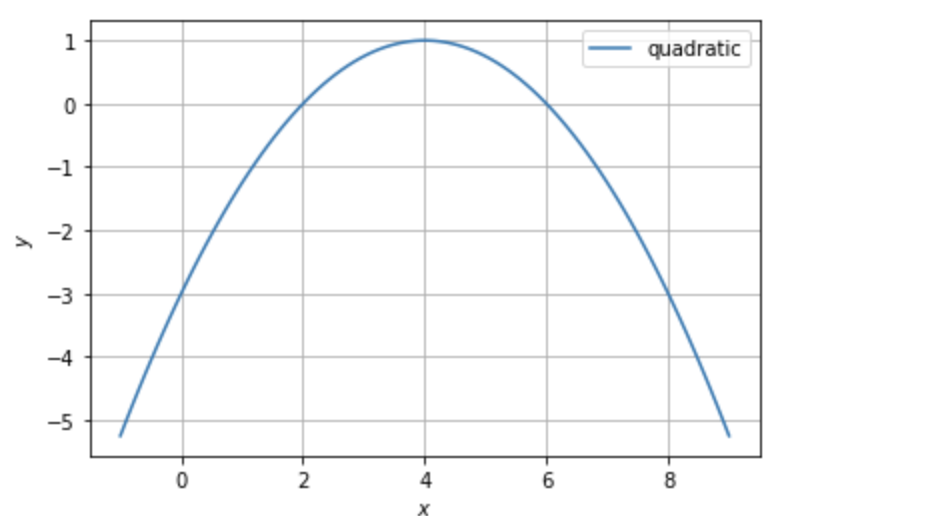
\includegraphics[width=\columnwidth]{5.1}
	  \caption{}
	  \label{fig:geometry-3.9.pdf}
 \end{figure}
\begin{align}
& 4k+4-3=0 \nonumber\\
& k = -\dfrac{1}{4} \nonumber 
\end{align}   

\item Find the values of $k$ for which the quadratic equation has $3x^2+kx+3 = 0$ has real and equal roots. \\
\solution For real and equal roots if an quadratic equation $ax^2+bx+c=0$, $b^2-4ac = 0$ \\
 \begin{figure}
	  \centering 
	  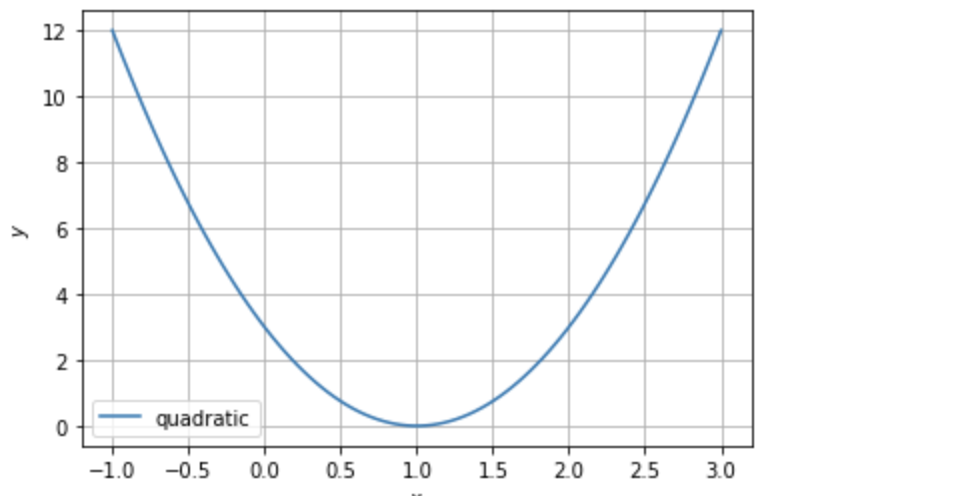
\includegraphics[width=\columnwidth]{5.2}
	  \caption{}
	  \label{fig:geometry-3.9.pdf}
 \end{figure}
\begin{align}
k^2-4*3*3 =0 \nonumber \\
k = \pm 6 \nonumber
\end{align}

\item A train travels 360 km at a uniform speed. If the speed had been 5 km/hr more, it would have taken 1 hour less for the same journey. Find the speed of the train. \\
 \begin{figure}
	  \centering 
	  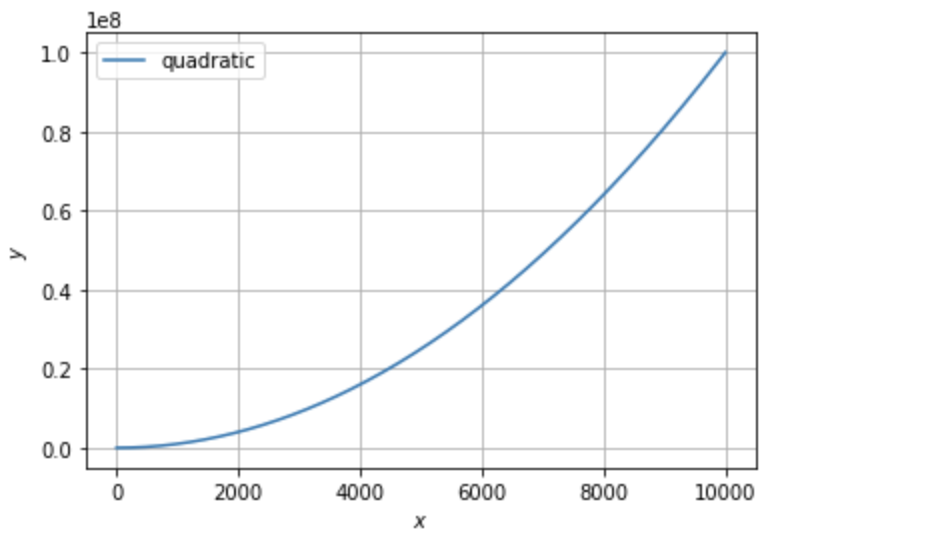
\includegraphics[width=\columnwidth]{5.3}
	  \caption{}
	  \label{fig:geometry-3.9.pdf}
 \end{figure}

\solution Let the speed of the train be s km/hr and the time taken be t hours.\\
Distance = Speed × Time \\
360 = s × t \\

$t = \dfrac{360}{s}$ \\
Increased speed of the train can be written as s + 5 \\
New time to cover the same distance = t - 1 \\
$(s + 5) × (t - 1) = 360$ \\
$st - s + 5t - 5 = 360$ \\

$360 - s + 5(\dfrac{360}{s}) - 5 = 360$\\

$s^2 + 5s - 1800 = 0$ \\ 
Simplifying the above equation we get, \\
s = 40 and s = - 45 \\
Speed of the train cannot be a negative value.\\
Therefore, speed of the train is 40 km /hr. \\

\item  Find all the zeroes of the polynomial $x^4+x^3-14x^2-2x+24$, if two of its zeroes are $\sqrt{2}$ and $-\sqrt{2}$. \\
 \begin{figure}
	  \centering 
	  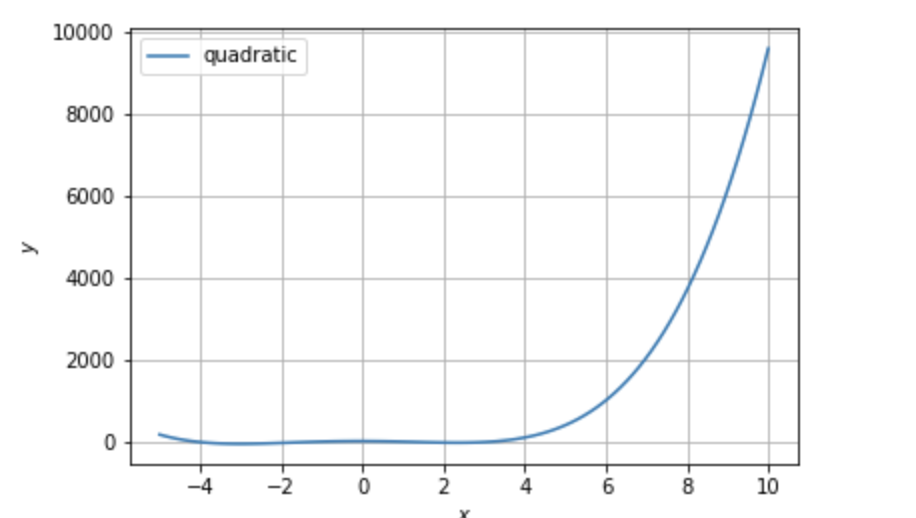
\includegraphics[width=\columnwidth]{5.4}
	  \caption{}
	  \label{fig:geometry-3.9.pdf}
 \end{figure}
\solution let $x^4+x^3-14x^2-2x+24$ be $f(x)$, Given $\sqrt{2}$ and $-\sqrt{2}$. are two zeroes of $f(x)$. \\

$x-\sqrt{2}, x+\sqrt{2}$ roots of $f(x)$ \\
$x^2-2$ is the factor of $f(x)$ \\

\polylongdiv{x^4+x^3-14x^2-2x+24}{x^2-2} \\
Therefore the roots of the polynomial equation are $(x^2-2)(x^2+x-12) = 0$ \\
$(x^2-2)(x+4)(x-3) = 0$ \\
Other zeroes are -4 and 3 \\

\item Solve for $x: \dfrac{1}{a+b+x} = \dfrac{1}{a} + \dfrac{1}{b} + \dfrac{1}{x}; a \neq b \neq $, 

$x \neq 0, x \neq -(a+b)$\\
\begin{align}
\dfrac{1}{a+b+x} - \dfrac{1}{x} = \dfrac{1}{a} + \dfrac{1}{b} \nonumber \\
\dfrac{-(a+b)}{xa+bx+x^2} = \dfrac{(a+b)}{ab} \nonumber \\
-ab = xa+bx+x^2 \nonumber \\
xa+bx+x^2+ab = 0 \nonumber \\
x(x+b)+a(x+b) = 0 \nonumber \\
x = -a ; x= -b \nonumber
\end{align}


\end{enumerate}
\end{document}
